\documentclass{scaffold/sigchi}
\usepackage{pifont} % Check marks
\newcommand{\cmark}{\ding{51}} % So we can use \cmark instead of \ding{51}
\newcommand{\xmark}{\ding{55}}

% Title
\def\plaintitle{Investigating How Different Modalities of Positive Reinforcement Influence the Formation of New Habits}

% Authors as plain text
\def\plainauthor{First Author, Second Author, Third Author,
  Fourth Author, Fifth Author, Sixth Author}
\def\emptyauthor{}
\def\plainkeywords{habit formation; behaviour change; chatbot; rewards; modalities; visual; audio; visual-audio.}
\def\plaingeneralterms{Documentation, Standardization}
  \usepackage{pgfplots}
  \pgfplotsset{compat=1.12}

% Use this section to set the ACM copyright statement (e.g. for
% preprints).  Consult the conference website for the camera-ready
% copyright statement.

% Copyright
\CopyrightYear{2017}
%\setcopyright{acmcopyright}
\setcopyright{acmlicensed}
%\setcopyright{rightsretained}
%\setcopyright{usgov}
%\setcopyright{usgovmixed}
%\setcopyright{cagov}
%\setcopyright{cagovmixed}
% DOI
\doi{http://dx.doi.org/10.475/123_4}
% ISBN
\isbn{123-4567-24-567/08/06}
%Conference
\conferenceinfo{CHI'18,}{April 21--26, 2018, Montreal, Canada}
%Price
% \acmPrice{\$15.00}

% Use this command to override the default ACM copyright statement
% (e.g. for preprints).  Consult the conference website for the
% camera-ready copyright statement.

%% HOW TO OVERRIDE THE DEFAULT COPYRIGHT STRIP --
%% Please note you need to make sure the copy for your specific
%% license is used here!
% \toappear{
% Permission to make digital or hard copies of all or part of this work
% for personal or classroom use is granted without fee provided that
% copies are not made or distributed for profit or commercial advantage
% and that copies bear this notice and the full citation on the first
% page. Copyrights for components of this work owned by others than ACM
% must be honored. Abstracting with credit is permitted. To copy
% otherwise, or republish, to post on servers or to redistribute to
% lists, requires prior specific permission and/or a fee. Request
% permissions from \href{mailto:Permissions@acm.org}{Permissions@acm.org}. \\
% \emph{CHI '16},  May 07--12, 2016, San Jose, CA, USA \\
% ACM xxx-x-xxxx-xxxx-x/xx/xx\ldots \$15.00 \\
% DOI: \url{http://dx.doi.org/xx.xxxx/xxxxxxx.xxxxxxx}
% }

% Arabic page numbers for submission.  Remove this line to eliminate
% page numbers for the camera ready copy
% \pagenumbering{arabic}

% Load basic packages
\usepackage{balance}       % to better equalize the last page
\usepackage{graphics}      % for EPS, load graphicx instead 
\usepackage[T1]{fontenc}   % for umlauts and other diaeresis
\usepackage{txfonts}
\usepackage{mathptmx}
\usepackage[pdflang={en-US},pdftex]{hyperref}
\usepackage{color}
\usepackage{booktabs}
\usepackage{textcomp}

% Some optional stuff you might like/need.
\usepackage{microtype}        % Improved Tracking and Kerning
% \usepackage[all]{hypcap}    % Fixes bug in hyperref caption linking
\usepackage{ccicons}          % Cite your images correctly!
% \usepackage[utf8]{inputenc} % for a UTF8 editor only

% If you want to use todo notes, marginpars etc. during creation of
% your draft document, you have to enable the "chi_draft" option for
% the document class. To do this, change the very first line to:
% "\documentclass[chi_draft]{sigchi}". You can then place todo notes
% by using the "\todo{...}"  command. Make sure to disable the draft
% option again before submitting your final document.
\usepackage{todonotes}






% llt: Define a global style for URLs, rather that the default one
\makeatletter
\def\url@leostyle{%
  \@ifundefined{selectfont}{
    \def\UrlFont{\sf}
  }{
    \def\UrlFont{\small\bf\ttfamily}
  }}
\makeatother
\urlstyle{leo}




% To make various LaTeX processors do the right thing with page size.
\def\pprw{8.5in}
\def\pprh{11in}
\special{papersize=\pprw,\pprh}
\setlength{\paperwidth}{\pprw}
\setlength{\paperheight}{\pprh}
\setlength{\pdfpagewidth}{\pprw}
\setlength{\pdfpageheight}{\pprh}

% Make sure hyperref comes last of your loaded packages, to give it a
% fighting chance of not being over-written, since its job is to
% redefine many LaTeX commands.
\definecolor{linkColor}{RGB}{6,125,233}
\hypersetup{%
  pdftitle={\plaintitle},
% Use \plainauthor for final version.
%  pdfauthor={\plainauthor},
  pdfauthor={\emptyauthor},
  pdfkeywords={\plainkeywords},
  pdfdisplaydoctitle=true, % For Accessibility
  bookmarksnumbered,
  pdfstartview={FitH},
  colorlinks,
  citecolor=black,
  filecolor=black,
  linkcolor=black,
  urlcolor=linkColor,
  breaklinks=true,
  hypertexnames=false
}

% create a shortcut to typeset table headings
% \newcommand\tabhead[1]{\small\textbf{#1}}

\title{\plaintitle}




% Authors on paper
\numberofauthors{3}
\author{%
  \alignauthor{Leave Authors Anonymous\\
    \affaddr{for Submission}\\
    \affaddr{City, Country}\\
    \email{e-mail address}}\\
  \alignauthor{Leave Authors Anonymous\\
    \affaddr{for Submission}\\
    \affaddr{City, Country}\\
    \email{e-mail address}}\\
  \alignauthor{Leave Authors Anonymous\\
    \affaddr{for Submission}\\
    \affaddr{City, Country}\\
    \email{e-mail address}}\\
}

\begin{document}

\maketitle

\begin{abstract}
Rewards motivate people to complete tasks. Habit formation systems use rewards to motivate people to form habits. This paper looks at the effect of habit formation using three types of positive reinforcement rewards from two modalities, visual, auditory and visual-auditory combined. We evaluate the findings against our two hypothesis: What is the effect of rewards on habit completion and strength; How do multiple modalities effect habit completion and strength. 60 people participated in a 4-week study followed by voluntary semi-structured interviews. Our findings show that participants receiving our bot-delivered rewards completed more habits than the control group. We also found a correlation between the our habit formation method and habit strength. However, all participants interviewed (N = 7) found a drop in habit performance after 1-week without our prototype. We outline the dangers in technology dependence and hope that our research provides new avenues for combing modalities and behaviour change for the HCI community.
\end{abstract}

\category{H.5.2}{Information interfaces and presentation (e.g. HCI)}{User Interfaces, auditory (non-speech) feedback, interaction styles}
\category{J.4}{Social and Behavioural Sciences}{Psychology}

\keywords{\plainkeywords}


\section{Introduction}
Using technology to form new habits is important to the HCI community. Habits require behaviour change interventions to become permanent. Understanding how we can build tech to action change means we know how to support behaviour change. Understanding the full habit formation process within tech needs further research.
It is difficult to evaluate the long-term effects of technology, due to the practical limitations of building technology that motivates people to adopt new habits~\cite{how_to_evaluate_tech_for_behaviour_change}. However, the need for HCI researchers to design technology that encourages people to change their behaviour is still main focus.

Psychology defines habits as learned automatic cue-response actions, such actions that will perform automatically in response to another action or trigger that has been actioned repeatedly in the past~\cite{article_the_habitual_consumer}. A simple action such as turning on the light to a room happens automatically, even if the light is already on. Forming a new habit is difficult, people normally give up, often due to their lack of routine~\cite{article_promoting_habit_formation, article_the_habitual_consumer}.

Technology can help people stick to a routine by sending repeated messages~\cite{chi_crowd_designed_motivation} and coaching that person along. However, these techniques do not always work~\cite{coaching_not_that_good}. Therefore, technology should be designed to avoid building repetitive actions and instead build habit strength. Repetitive actions lead people to become dependent on technology, and when the system is eventually removed, habit performance decreases~\cite{article_dont_kick_habit}. Habit automaticity is a measure of habit strength and is the key that removes this dependency~\cite{article_beyond_self_tracking_designing_apps}. Automaticity can be increased by building motivation to complete the action~\cite{article_a_self_efficacy, article_meta_analytic_review_intrinsic_motivation}.
Motivation can be encouraged by rewarding users with positive reinforcement after they complete the action.
However, these are not enough to be successful, the reward and delivery type are crucial to success.

The type of reward can effect motivation. Monetary rewards (extrinsic rewards) can hinder motivation~\cite{article_meta_analytic_review_intrinsic_motivation}, whereas, satisfaction-based rewards (intrinsic rewards) can be beneficial to motivation and should be preferred~\cite{article_meta_analytic_review_intrinsic_motivation}.
How rewards are delivered is also important. The method of delivery should suit each individual user, and a choice of delivery should be available. For example, research~\cite{article_user_centred_multimodal_reminders} into reminder systems shows that reminders should span different modalities to increase user retention and better suit the users needs.
We experiment with this new method of delivering rewards in the form of a bot sending intrinsic positive reinforcement rewards from different modalities to see how this affects people's habit strength.

In this paper we make three contributions. First, we present analysis of a 4-week situated study measuring the impact of visual, auditory and visual-auditory rewards on participants habit strength and the number of habits competed. Second, we show how our bot-delivered rewards encourage people to stick to a routine and perform their habit. Lastly, we demonstrate how our method of tracking habits increases habit strength, however, we discuss the dependency issues arising with technology and habit formation.

\section{Background}
\subsection{Mediation of Habit Formation}
Habits are automatic actions that require little concious effort~\cite{article_the_habitual_consumer}. To develop new habits people must keep to a strict strategy and perform the action repeatedly to strengthen the automaticity of the action~\cite{article_promoting_habit_formation}. When strong habits are developed the likelihood of behaviours persisting is higher~\cite{putting_habit_into_practice}. The formation of new habits requires behaviour change. Three elements are needed to make this change permanent: repetition, contextual cues and positive reinforcement~\cite{article_experiences_of_habit_formation}. Positive reinforcement rewards the person by encouraging them to perform the action again until it forms into a habit. This has been shown to significantly increase intrinsic motivation and increase in the persons perception of their own performance~\cite{positive_reinforcement_pro}. Finally, repetition is needed --- as habits, on average, take up to 66 days to form~\cite{article_how_habits_formed_modelling_habit_formation}.
However, people still fail at forming new positive habits and give up, often due to their lack of routine~\cite{article_promoting_habit_formation, article_the_habitual_consumer}.



\subsubsection{Repetition \& Cues}
The process of creating a new habit takes on average 66 days of repetitive use~\cite{article_how_habits_formed_modelling_habit_formation}. The easier the action, the shorter time before the action turns into a habit, from drinking water (18 days), to going to the gym (254 days). However, existing routines and cues are needed before the action develops into a habit. An existing routine acts as a trigger to motivate the desired action. Context from that routine serves as the cue for the trigger. For example, if you wanted to adopt a stretching habit, you could attach it onto an existing habit like (waking up). The contextual cue of brushing your teeth will trigger you to stretch. Attaching habits onto existing event-based cues are easier to remember~\cite{article_implementation_intentions_multicue}, when compared with time-based habits, e.g. stretch every 4 hours, or at a specific time as these times usually change with changes in environment, e.g. weekend~\cite{coaching_not_that_good}. Event-based cues help connect the contextual information with the action and builds habit automaticity~\cite{article_implementation_intentions}. Finally, when designing behaviour change interventions multi-cue routines have shown to be more effective than a single cue~\cite{article_understanding_use_contextual_cues_design_impl}.

\subsubsection{Rewards}
Self-efficacy (the belief in ones ability to succeed) plays a large part in forming habits~\cite{article_a_self_efficacy} and some research suggests it is the main part of behaviour change. Rewards give people this experience by feeding back their success of their action. Rewarding a person with positive reinforcement, strengthens the habit by giving the feeling of satisfaction~\cite{article_promoting_habit_formation}. However, the type of reward matters, as rewards that benefit the person with satisfaction (intrinsic rewards) should be used over monetary gains (extrinsic rewards), because extrinsic rewards have a negative effect on motivation~\cite{article_meta_analytic_review_intrinsic_motivation}, particularly in relation to interesting tasks. Therefore, this paper focuses on positive reinforcement intrinsic rewards.



\subsection{Positive Reinforcement}
TODO: Compare different reward types. We will focus only on positive reinforcement rewards, however, there are lots of different types...

TODO: Reward rationale, stating the rise of social media, with memes, these rewards seem appropriate for a chatbot.

TODO: Reword this para, duplicated reward and awkward) Previous habit formation research~\cite{article_understanding_use_contextual_cues_design_impl} shows how different \textit{contextual cues} better support behaviour change, compared with a single mode. But, we want to see if using different types of \textit{positive reinforcement} rewards better supports behaviour change, compared with single mode. We want to map habit rewards across different modalities, to present users with the same reward type from a different modality.
This allows us to test the different types of modalities and how they effect behaviour change.
The next section discusses methods of interaction in practice.

\subsection{Modalities}
The three chosen modes, visual, auditory, and visual-auditory combined, are chosen for testing. Feedback from each of these different modalities, has been shown to impact the task performance for small tasks~\cite{chi_oussama_tap_the_shapetones}. TODO join the next paragraphs into this one.


(dont have quotes, reword section, sounds awkward whole thing) `Multi-modal systems are required for user interaction'~\cite{article_user_centred_multimodal_reminders} states research into comparing uni-modal reminders systems with multi-modal.
They suggests a need for `highly flexible and contextualised multi-modal and multi-device reminder systems'~\cite{article_user_centred_multimodal_reminders}.
Although this study focused on the elderly, so the need to multiple modalities was important because some peoples sensory modalities decline with age,
this principle still holds true for general case reminder systems. The study presents design guidelines for reminder systems.
These are mainly focused on users needing a choice of modalities for interacting with users, as users want a highly configurable system.

Research into designing (reminder systems)? for the home that interact with users in different modalities, states that
`Good reminder systems should use different modalities, because they provide alternative ways to interact with a user'~\cite{article_designing_multimodal_reminders_for_home}.
Using different modalities for interaction increases the likelihood that the information users are receiving will be more receptive to them,
and decreases the chance the interaction will be disruptive or annoying~\cite{article_designing_multimodal_reminders_for_home}.
Habit rewards should not be annoying, they should give users a feeling of satisfaction, therefore reducing the chance of disruption is another justification for using multiple modalities.

We want to compare each modality with a control group to see how habit formation is impacted. The next section looks at literature discussing visual, audio and visual-audio modality types used and how they change peoples behaviour.

\subsubsection{Visual}
(add other studies)
This habit-forming system used visual feedback to encourage consistency...
One study looked at improving habit consistency for how often patients took medication,
by using a visual display device that gave constant feedback~\cite{article_realtime_feedback_improving_medication_taking}.
They found that this feedback improved consistency of the habit and increasing rating of self-efficacy.
But when the device was removed, their performance dropped (from a 2-month follow up study), because users integrated the feedback display with their routines.
However, this system shouldn't integrate visual cues into the system, otherwise users become dependent on the technology.
Users should instead build these cues outside of the system to build performance longevity after removing the system.

\subsubsection{Auditory}
(reword start, awkward)
Another key paper discussed their need for different modalities when designing for the elderly~\cite{article_movipill_improving_medication_elders},
combing different sounds with high visual contrast to suit their needs, given deteriorating senses due to age.
The study showed that using a combination of modalities for interaction gives a means of communication to people with varying levels of sense ability.
But studies have also shown people need a choice of mode when designing for interaction~\cite{article_user_centred_multimodal_reminders},
and thus the design requirements produced from this study can be applied to general applications that use multiple modalities, such as this project.
The design guidelines discuss the need for interaction consistency, such as using similar audio interaction.
Therefore visual and auditory rewards are mapped identifying a pattern across the modalities.

\subsubsection{Visual-Auditory}
Talk about vauge combining modalities, then focus in on v a

Combining audio with visual can be advantageous as feedback after the completion of a simple task, as proven by lots of research, e.g.~\cite{benefits_of_audio_visual_1, benefits_of_audio_visual_2}. A meta-analysis of 43 multi-modal studies~\cite{comparing_modalities_effects_of_visual_auditory} revealed that it was the most effective to increase performance, when a single task is being performed, when compared with visual or auditory feedback alone. However, care needs to be taken when adding an extra modality as this research states that 'visual feedback improved task performance, but not error rate'~\cite{comparing_modalities_effects_of_visual_auditory}. In addition, while all modalities contribute to perceptual experience, one sense can override another if the sensory channel mediates less ambiguous information than the other~\cite{one_mode_override_another}. Finally, this combination of visual and auditory sensory channels has been shown to increase performance with complex tasks~\cite{chi_oussama_tap_the_shapetones}, therefore it will be useful to compare the success of the task with the other modes.

These aspects are implemented into our prototype and adapted for delivering rewards.

\subsection{Mapping Modalities}
First, the actual rewards are aimed to motivate participants to complete further habits. Gifs and audio are found from the site, with the search 'Motivation'. Each frame of the gif image is altered to match the audio frequency level. The frame is slowed down if the audio level is lower, or speed up, if the audio frequency level is higher. The relationship between the audio and the visual is inferred, therefore this mapping is \textit{semi-congruent}. The next section discusses how technology is used to create a delivery method for these rewards.

\section{Technology}



Research~\cite{survey_on_apps_2,survey_on_current_apps_of_steel} into how mobile systems can support habit formation and behaviour change, shows a large number of habit forming systems are mobile apps. Studies into the effectiveness of these apps has been recently conducted~\cite{article_beyond_self_tracking_designing_apps, article_dont_kick_habit} revealing that although most of these apps are rated highly, they do not ground themselves in behaviour change theory. Research into some of these apps show that habits are not sustained when the app is removed, due to the lack of habit automaticity~\cite{article_beyond_self_tracking_designing_apps}.

Two pieces of literature discuss different strategies for building habit forming mobile systems that do ground themselves in theory: Stawarz et al.~\cite{article_beyond_self_tracking_designing_apps} discuss guidelines for building habit forming apps and Weiser et al.~\cite{article_taxonomy_motivational_affordances_meaningful} show that `motivation is a key requirement for behaviour change' presenting five design principles and six requirements about the implementation mechanics of habit forming systems that focus on rewards and motivational needs. These share three recommendations: i) make personalized, well-defined, structured multi-cue routines, with examples, \& support users choice of not setting remembering strategies, ii) reminders can effectively support prospective memory in the short-term, increase the logging of health data~\cite{the_power_of_logging_mobile_notifications} and educate them about what they should perform in the long-term, iii) Rewards are a good form of external motivation because they don't change the ability to perform a behaviour, unless the reward itself is a tool that increases ability. These rewards provide a strong motivational source, but like all extrinsic motivators, these are less effective for changing behaviour in the long run, because externally motivated behaviour lasts as long as the external motivator exists.

Technology can help people stick to a routine. By associating the desired action with contextual information to develop a cue. It can positively reinforce with rewards after completing the action. Finally, it can send repetitive notifications, that adjust to changes in environment.
Yet most existing habit formation systems are not always built on theory~\cite{article_beyond_self_tracking_designing_apps}, and usually build repetitive actions rather than habit automaticity.
Therefore, people become dependent on technology, and when the system is eventually removed, habit performance decreases~\cite{article_dont_kick_habit}. Building habit automaticity is the key that removes this dependency~\cite{article_beyond_self_tracking_designing_apps}.

Interaction with current habit formation systems is often via a mobile app. This creates a notable difference in the person when the system is removed~\cite{article_my_phone_is_part_of_my_soul}.
This is also the case with many mobile feedback systems that aid with behaviour change.
When we remove the system any improved performance is lost~\cite{article_dont_kick_habit, article_realtime_feedback_improving_medication_taking}. To build a system for mobile devices that meets our requirements we must review all available options. A chatbot can easily send notifications, has a short development time, high availability with cross-platform and is simple, with the UI already built for us.

TODO somewhere here We need a bot to deliver the positive reinforcement because (summarise the table that we deleted).



\begin{figure}
  \centering
  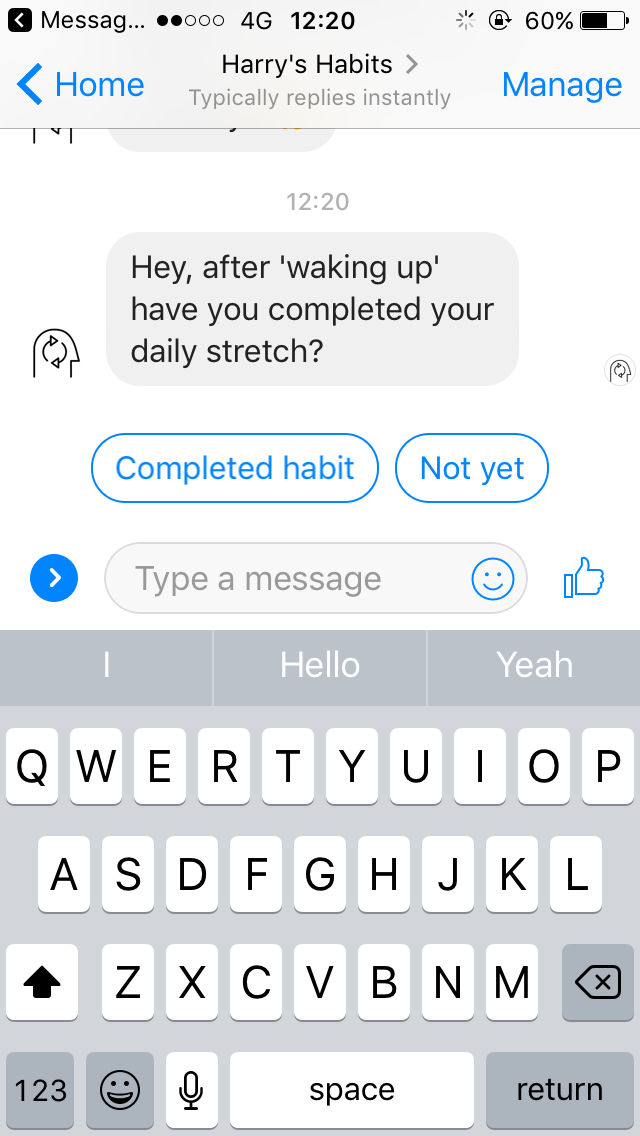
\includegraphics[width=0.47\columnwidth]{figures/reminder.png}
  \hspace{5px}
  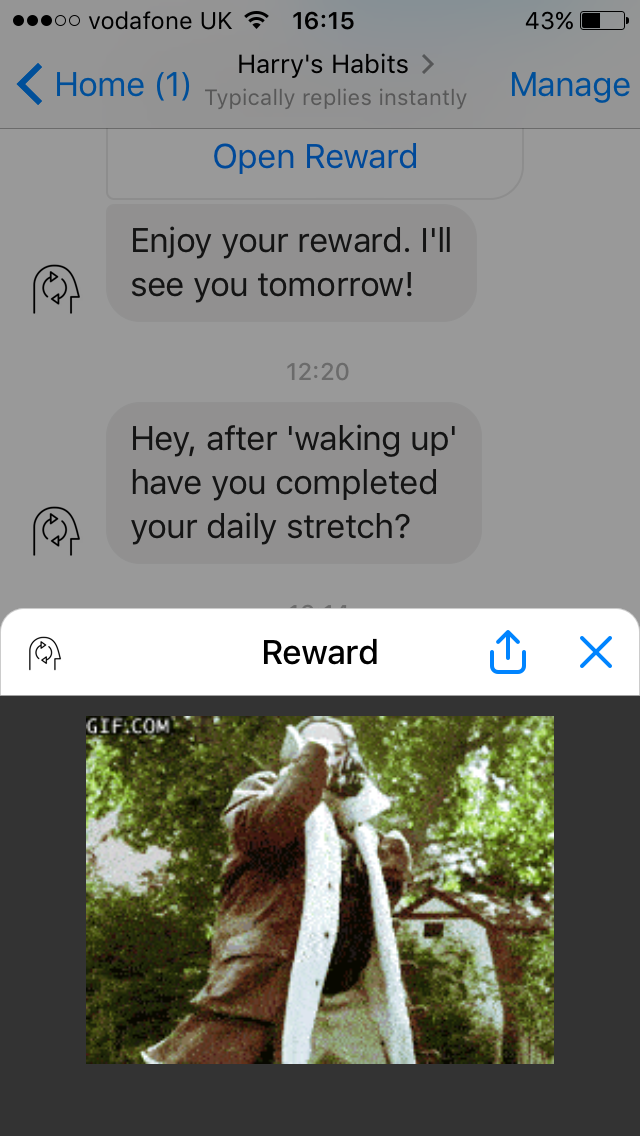
\includegraphics[width=0.47\columnwidth]{figures/reward-visual.png}
  \caption{Prototype delivering a visual reward after a user has marked their habit as completed.}~\label{fig:setup}
\end{figure}

\section{Study: Comparing Different Rewards}
To explore the influence of different modalities on habit formation, we would conducted a something study, followed by semi-structured interviews. For the purpose of the study we developed a chatbot that helps users form healthy habits by providing different types of positive reinforcement. The study and the bot itself are described below.



\subsection{Method}
The study aims to test 2 hypothesis to compare how well people form new habits based on their reward modality and how the rewards delivered by the chatbot effect participants habit formation.

\subsubsection{Hypothesis}
H1: Are rewards better than no rewards: Compare all aggregated reward modalities with control group (no rewards).


H2: Are multiple modalities better than a singular mode: Compare Visual-Audio with Visual, Audio aggregated.

\subsubsection{Conditions}
C1: Habit Strength: Calculated based on two SRHI questionnaires.


C2: Number of Completed Habits: Number incremented when a participant presses '\textit{Completed habit}'.

\subsubsection{Participants}
60 participants were recruited on social networks (using the landing page: \url{www.harrymt.com/harryshabits}), and were mostly University students and staff. They were instructed to connect with the bot via Facebook Messenger and pick a series of options to set-up their habit tracking.



\subsubsection{Design}


\begin{table}
  \centering
  \begin{tabular}{l l l}
    % \toprule
    {\small\textit{Modality}} & {\small \textit{Reward}} & {\small \textit{No. Participants}}\\
    \midrule
    Visual & 15s gif & 15 \\
    Auditory & 15s audio & 15 \\
    Visual \& Auditory & 15s gif and audio & 15 \\
    None (control group) & No reward & 15 \\
    % \bottomrule
  \end{tabular}
  \caption{Participants are split into these four study conditions.}~\label{tab:precise_rewards}
\end{table}

A brief description accompanied these questions, to guide the participants on how to answer. The habits participants could choose were split into two categories, physical and relaxation. They were: stretching, press ups, the plank, reading, writing or meditation.\newline
\newline
The study used four conditions: visual rewards, auditory rewards, visual-auditory rewards and no rewards (control group). Participants were randomly assigned a condition by the bot after they completed the set-up, 15 were assigned with visual rewards, 15 assigned audio rewards, 15 assigned visual-audio and 15 assigned no rewards (control group).\newline
\newline
Participants would receive a confirmation message, followed by positive reinforcement after they marked a habit as complete, unless they were in the control group, then they would only receive a confirmation message.


\subsubsection{Materials}
The bot will collect the amount of habits people complete verses their reward type. Habit completion will be verified by using the SRBAI questionnaire~\cite{article_habit_measurement}---A validated set of questions to measure habit automaticity levels. This will be used to test if people are forming a habit. Finally, participant interviews will discuss the chatbot delivered rewards for further verification.

A subset (4-questions) of the SRHI~\cite{article_habit_strength}  to measure habit automaticity levels

Likert scale was also used for various questions about participant rewards coined a modality survey.
 
\begin{figure}
  \centering
  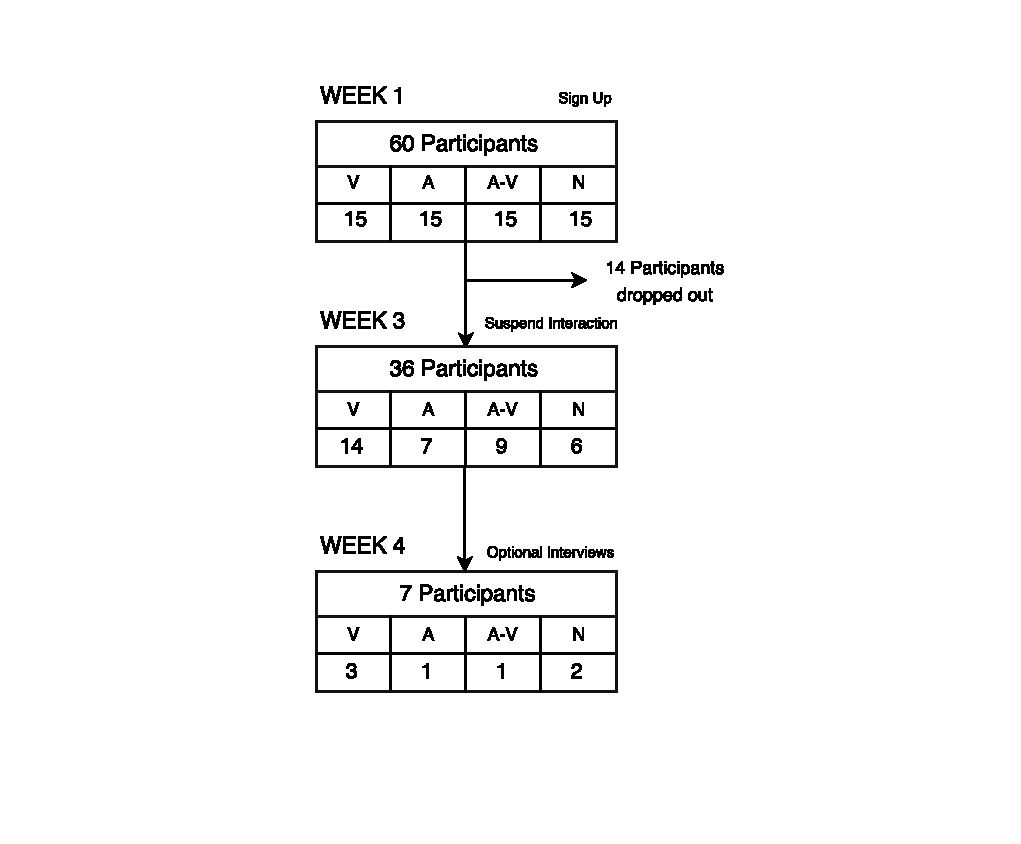
\includegraphics[width=.8\columnwidth]{figures/study-flow}
  \caption{Study overview.}~\label{fig:study_flow}
\end{figure}
 
\subsubsection{Procedure}
First, we conducted an internal pilot trial to develop the strength of the prototype. Second, we ran a 4-week evaluation trial in the wild with real people who try and form a new positive habit. Finally, follow-up interviews with participants test if they continued with their habit without the bot.\newline
\newline
The 4-week evaluation trial is split into two sections. First a 3-week trial tests the success of the chatbot by evaluating the tool and the effectiveness of each modality on participants habit strength using a validated questionnaire~\cite{article_habit_measurement}. During the fourth week, chatbot interaction is removed during a 1-week follow up trial to test if participants continue with the habit. Participants were split into four groups, all groups receiving reminders, three groups receiving rewards each from a different modality, and one group (control group) don't receive any rewards.


At the beginning of the 3-week period, participants were asked to answer basic demographic information and choose a new habit they would like to develop from a list of habits of similar difficulty, divided into two categories: physical and relaxation. Then they were asked to state an existing routine they could build their new habit around, and choose a time that routine normally occurred (Morning, Afternoon, Evening). After they had answered these questions, they would be auto assigned a modality (unknowingly to users) for rewards, and they would continue with their day. Participants would complete their chosen habit every day after their existing routine, then wait for the bot to send them a message asking them for one of two choices.\newline
\newline
Option one (completed habit): participants would receive a message thanking them, then participants not in the control group would receive a message linking them to a reward. This reward would be from the modality auto-assigned to that participant during the set-up phase (table~\ref{tab:precise_rewards}). Option two (not yet): the bot would check on the participant an hour later. This allowed for the checks to be snoozed, to ensure the new habit fit in with participants routine. If participants constantly told the bot they hadn't completed their habit yet, the bot would ask participants if they would like to change the time their routine occurred. This allowed the participants in the beginning to refine the time they would perform their habit.

After 3 weeks of participants interacting with the bot, all participants who completed the set up are asked to complete the SRHI~\cite{article_habit_strength} questionnaire. Then the bot interaction was suspended for 1 week. After the full 4-week period, participants were asked to complete the questionnaire again. Both questionnaires presented the questions on a 7-point Likert scale with answers from 'Strongly Disagree' (5) to 'Strongly Agree' (1). Higher scores indicates higher self-reported levels of automaticity. In addition, participants had an option to opt-in for an interview about their experience after the 4-week period.

\section{Results}
60 participants connected with the bot by pressing \textit{'Get Started'} in Facebook Messenger on the following platforms: 25 browser, iOS 18 and Android 12. 14 people (23\%) dropped out of the study at various stages: 54 people (90\%) continued interacting with the bot and started the set-up. 39 people (65\%) completed the set-up and out of these 39 people, 3 people just ignored all messages from the bot during the trial. Leaving 36 participants (66\%) that are considered active throughout and included in the final analysis. These 36 participants are 18-63 years old, (mean: 27 years old, SD: 12), 23 (64\%) male, 11 (30\%) female and 2 (6\%) didn't say. These 36 remaining participants are split into the following modalities: 14 people (93\%) visual, 9 people (60\%) visual and auditory, 7 people (46\%) auditory and 6 people (40\%) had no rewards (control group). 28 participants volunteered for an interview (at the beginning of the study, but only 7 participants arranged a time for one,) and 7 were carried out.


\subsection{General Trend}
36 participants sent a total of 1.1k messages to the bot (mean = 65 messages per participant) and the bot sent 2.7k total messages back. 184 total habits were marked as completed, with the bot issuing 69 visual rewards, 58 visual-auditory rewards and 17 auditory rewards to those participants. The control group completed 40 habits and were sent 0 rewards. Out of the 36 participants, 4 people blocked/deleted the thread during the study, 6 people blocked/deleted thread at the end of the 3-week period, after the bot messaged all users 'See you in a week'. Their data is included in this analysis.


Comparing the number of people who dropped out of the study verses their reward modality, we see that 7 participants who blocked the bot had 27 visual rewards in total (mean = 3.85). 2 participants had 4 total auditory rewards (mean = 2) and 2 participants had 2 visual-auditory combined (mean = 6.5). These visual-auditory participants that dropped out had the highest amount of snoozes (24 total snoozes, 6 and 18 individually, mean = 12), compared with visual 10 total (mean = 2), and auditory with 0 snoozes.


7 participants (19\%) previously used habit tracking systems and 100\% of stated they worked well for tracking habits. These habits were: 'Diet' (3 mentions), 'Exercise' (3 mentions), 'Deadlines' (2 mentions), 'Audiobook reading' (1 mention), 'Weight' (1 mention). All of these participants chose new habits that they hadn't tracked before. Meditation was the most popular habit chosen (12 people 33\%), followed by Press ups (8 people 22\%), then Stretching (6 people 15\%). Reading and writing were the least, only selected by 4 and 2 people respectively. Stretching (6 people 15\%) was the most completed habit based on selection (60 times), ranking 10.0 (where 10.0 = 60/6). Meditation ranked 6.25 (6.25 = 75/12) and the least were the plank and reading with 3.75 (15/4) and 1.75 (7/4) respectively.


Participants (14 people 39\%) with visual rewards had the highest total number of snoozes (72 total presses to 'Not Yet'), auditory had the smallest (14 total). The control group had 55 snoozes and visual-auditory had 45 snoozes. Most people snoozed (answered 'Not Yet') in the morning (100 times), specifically mid (66) and late (27) morning. Visual and sound had the most number of failed snoozes (10, split over 6 people, 1 person had 5 failed snoozes). Then it was sound by 4.


Habit performance was also tracked in the form of a streak. If a participant did not track a habit for a day, their streak would be reset to 0. Meditation had the most cumulative streak (17) followed by stretching (7 people). High streaks (streak > 10) had habits: meditation (total 135 streaks) and stretch (126 streaks). Visual-Auditory rewards had the most streaks (126 combined), control group had 75, then Visual had 60. Stretch had the highest peak streak (18), meditation (15). However, overall, for all habits completed, meditation was the most streaked (269 combined), stretching (231 combined), then press ups (39) then plank (24).

\subsection{C1: Habit Strength}
11 participants completed both SRHI questionnaires, 2 control group, 2 auditory, 5 visual and 2 visual-auditory. A paired-samples t-test was conducted to evaluate the change of habit strength between the first SRHI questionnaire (after 3 weeks) and the second (after 4 weeks). We found there was a statistically significant increase in automaticity scores from SRHI 1 (mean = 14.18, SD = 3.78) to SRHI 2 (mean = 15.09, SD = 4.34), t (10) = 2.469, p <. 0005 (two-tailed). The mean increase in SRHI scores was 0.90 with a 95\% confidence interval ranging from 0.08 to 1.72. The eta squared statistic (.37) indicated a large effect size.

\subsubsection{C1H1: rewards verses control group}

% 			S1 Mean	S2 Mean	S1 SD		S2 SD
% Control	13.5	14.5	4.949747468	6.363961031
% Rewards	14.33	15.22	3.840572874	4.294699576

\begin{figure}
  \centering
 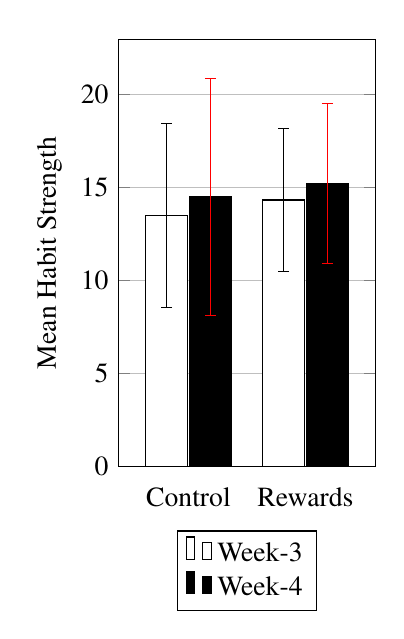
\begin{tikzpicture}
   \begin{axis}[
      width  = 0.4*\textwidth,
      height = 7cm,
      major x tick style = transparent,
      ybar=2*\pgflinewidth,
      bar width=15pt,
      ymajorgrids = true,
      symbolic x coords={Control,Rewards},
      xtick = data,
      scaled y ticks = false,
      enlarge x limits=0.60,
      ymin=0,
      legend cell align=left,
      legend style={at={(0.5,-0.15)},anchor=north},
%       x label style={at={(axis description cs:0.5,-0.1)},anchor=north},
%       y label style={at={(axis description cs:-0.1,.5)},rotate=90,anchor=south},
%       xlabel={$u$ unemployment},
      ylabel={Mean Habit Strength},
   ]
      \addplot[style={fill=white},error bars/.cd, y dir=both, y explicit]
          coordinates {
          (Control, 13.5) += (0,4.94) -= (0,4.94)
          (Rewards, 14.33) += (0,3.84) -= (0,3.84)
          };

      \addplot[style={fill=black},error bars/.cd, y dir=both, y explicit,error bar style=red]
           coordinates {
           (Control, 14.5) += (0,6.36) -= (0,6.36)
           (Rewards, 15.22) += (0,4.29) -= (0,4.29)
           };

      \legend{Week-3, Week-4}

  \end{axis}
  \end{tikzpicture}
  \caption{C1 H1: Comparing mean habit strength for rewards and control group.}~\label{fig:habit_4_item_survey1_v_survey2}
\end{figure}

An independent-samples t-test was conducted to compare the habit automaticity scores
for rewards and control at both SRHI 1 and SRHI 2. For SRHI 1, there was also no significant differences in scores for rewards (mean = 14.33, SD = 3.84) and control (mean = 13.50, SD = 4.94; t (9) = 0.224, p = .85,
two-tailed). The magnitude of the differences in the means (mean difference = .83,
95\% CI: \-29.43 to 27.76) was very small (eta squared = .005). For SRHI 2, there was no significant difference in scores for rewards
(mean = 15.22, SD = 4.29) and control (mean = 14.50, SD = 6.36; t (9) = 0.202, p = .84,
two-tailed). The magnitude of the differences in the means (mean difference = .72,
95\% CI: \-8.80 to 7.36) was very small (eta squared = .004).


A one-way between-groups analysis of variance with planned comparisons was also conducted to explore the impact of rewards on habit strength, as measured by the SRHI 1 and 2. Participants were divided into two groups (Group 1: visual rewards, auditory rewards, visual-auditory rewards combined; Group 2: control group. There was not a
statistically significant difference for the two groups at SRHI 1: F (1, 9) = 0.02, p = .88, and SRHI 2: F (1, 9) = 0.07, p = .78. In addition, the difference in mean scores between the groups had, at SHRI 1: a medium effect with an effect size of .11, and at SRHI 2: a large effect, with an effect size of .17, both calculated using eta squared.

\subsubsection{C1H2: multiple modalities verses singular mode}

% 			S1 Mean	S2 Mean	S1 SD	S2 SD
% Visual	14.6	15.8	4.336	3.701
% Auditory	12		11.5	4.243	6.364
% V-A		16		17.5	2.828	3.536

\begin{figure}
  \centering
 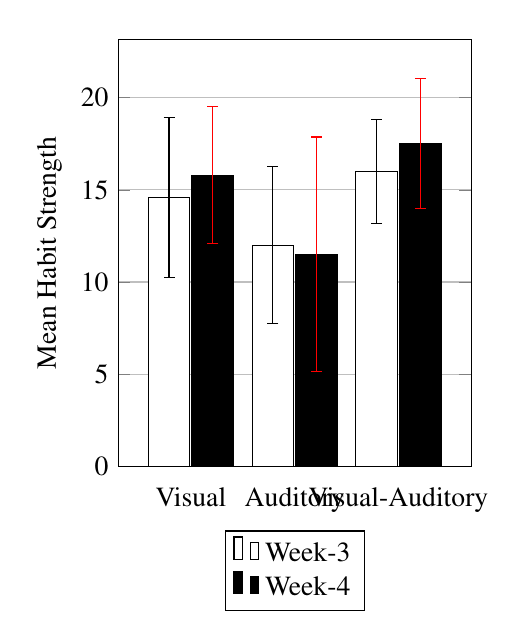
\begin{tikzpicture}
   \begin{axis}[
      width  = 0.5*\textwidth,
      height = 7cm,
      major x tick style = transparent,
      ybar=2*\pgflinewidth,
      bar width=15pt,
      ymajorgrids = true,
      symbolic x coords={Visual,Auditory,Visual-Auditory},
      xtick = data,
      scaled y ticks = false,
      enlarge x limits=0.35, % how far apart the bars are
      ymin=0,
      legend cell align=left,
      legend style={at={(0.5,-0.15)},anchor=north},
%       x label style={at={(axis description cs:0.5,-0.1)},anchor=north},
%       y label style={at={(axis description cs:-0.1,.5)},rotate=90,anchor=south},
%       xlabel={$u$ unemployment},
      ylabel={Mean Habit Strength},
   ]
      \addplot[style={fill=white},error bars/.cd, y dir=both, y explicit]
          coordinates {
          (Visual, 14.6) += (0,4.336) -= (0,4.336)
          (Auditory, 12) += (0,4.243) -= (0,4.243)
          (Visual-Auditory, 16) += (0,2.828) -= (0,2.828)
          };

      \addplot[style={fill=black},error bars/.cd, y dir=both, y explicit,error bar style=red]
           coordinates {
          (Visual,15.8) += (0,3.701) -= (0,3.701)
          (Auditory, 11.5) += (0,6.364) -= (0,6.364)
          (Visual-Auditory, 17.5) += (0,3.536) -= (0,3.536)
           };

      \legend{Week-3, Week-4}

  \end{axis}
  \end{tikzpicture}
  \caption{C1 H2: Comparing mean habit strength for rewards and control group.}~\label{fig:habit_4_item_survey1_v_survey2}
\end{figure}

A one-way between-groups analysis of variance with planned comparisons was conducted to explore the
impact of multiple modalities on habit strength, compared with singular modes as measured by the SRHI 1 and 2. Participants were divided into two groups according to their reward mode (Group 1: visual rewards, auditory rewards; Group 2: visual-auditory combined rewards). There was not a
statistically significant difference for the two groups at SRHI 1: F (1, 9) = 1.04, p = .33, and SRHI 2: F (1, 9) = 0.64, p = .44. In addition, the difference in mean scores between the groups had, at SHRI 1: a medium effect with an effect size of .11, and at SRHI 2: a large effect, with an effect size of .17, both calculated using eta squared.

\subsection{C2: Habits Completed}

\subsubsection{C2H1: rewards verses control group}

\begin{figure}
  \centering
 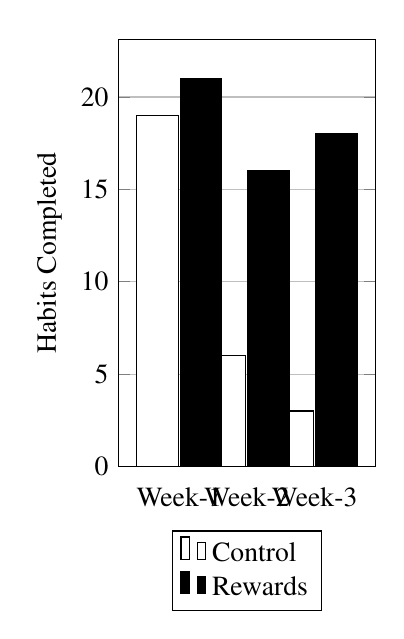
\begin{tikzpicture}
   \begin{axis}[
      width  = 0.4*\textwidth,
      height = 7cm,
      major x tick style = transparent,
      ybar=2*\pgflinewidth,
      bar width=15pt,
      ymajorgrids = true,
      symbolic x coords={Week-1, Week-2, Week-3},
      xtick = data,
      scaled y ticks = false,
      enlarge x limits=0.45,
      ymin=0,
      legend cell align=left,
      legend style={at={(0.5,-0.15)},anchor=north},
      ylabel={Habits Completed},
   ]
      \addplot[style={fill=white},error bars/.cd, y dir=both, y explicit]
          coordinates { % Control group
          (Week-1, 19)
          (Week-2, 6)
          (Week-3, 3)
          };

      \addplot[style={fill=black},error bars/.cd, y dir=both, y explicit,error bar style=red]
           coordinates { % Rewards
          (Week-1, 21)
          (Week-2, 16)
          (Week-3, 18)
           };

      \legend{Control, Rewards}

  \end{axis}
  \end{tikzpicture}
  \caption{Sum of completed habits for rewards and control group during 3-week study period.}~\label{fig:c2_h2}
\end{figure}

A one-way between-groups analysis of variance with planned comparisons was conducted to explore the effect of rewards on the number of habits completed, compared with control group. Participants were divided into two groups according to their reward mode (Group 1: visual rewards, auditory rewards, visual-auditory rewards; Group 2: control group). There was a statistically significant difference at the p < .005 level in both groups for two thirds of the Weeks: Week 1, F (1, 23.20) = 9.48, p = .005, Week 2, F (1, 33.35) = 4.46, p = 0.42 and Week 3, F (1, 50) = 17.01, p < 0.005. The effect size for Week 1, Week 2 and Week 3 are large, calculated using eta squared, were 0.25, 0.39 and 0.43 respectively, this shows a large difference in the mean scores.

\subsubsection{C2H2: multiple modalities verses singular mode}

A one-way between-groups analysis of variance with planned comparisons was conducted to explore the effect of multiple modalities and singular modalities on the number of habits completed. Participants were divided into two groups according to their mode (Group 1: visual rewards, auditory rewards; Group 2: visual-auditory rewards). There was a statistically significant difference at the p < .005 level in Week 2 and Week 3, and lots in all groups: Week 1, F (1, 50) = 0.69, p = .410, Week 2, F (1, 50) = 23.04, p < 0.005 and Week 3, F (1, 50) = 8.85, p = 0.005. The effect size for Week 1, Week 2 and Week 3 are large, calculated using eta squared, were 0.25, 0.39 and 0.43 respectively, this shows a large difference in the mean scores.

\begin{figure}
  \centering
 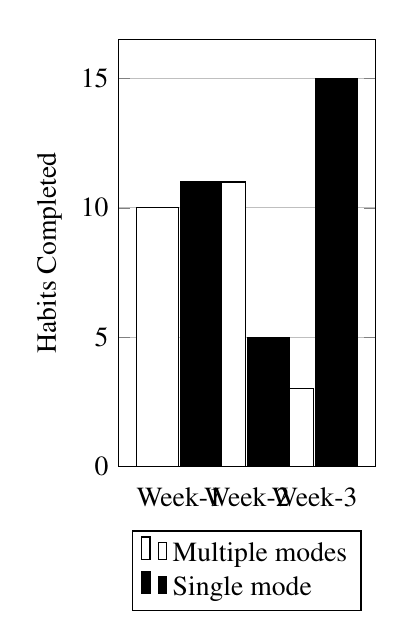
\begin{tikzpicture}
   \begin{axis}[
      width  = 0.4*\textwidth,
      height = 7cm,
      major x tick style = transparent,
      ybar=2*\pgflinewidth,
      bar width=15pt,
      ymajorgrids = true,
      symbolic x coords={Week-1, Week-2, Week-3},
      xtick = data,
      scaled y ticks = false,
      enlarge x limits=0.45,
      ymin=0,
      legend cell align=left,
      legend style={at={(0.5,-0.15)},anchor=north},
      ylabel={Habits Completed},
   ]
      \addplot[style={fill=white},error bars/.cd, y dir=both, y explicit]
          coordinates { % Multiple Modes
          (Week-1, 10)
          (Week-2, 11)
          (Week-3, 3)
          };

      \addplot[style={fill=black},error bars/.cd, y dir=both, y explicit,error bar style=red]
           coordinates { % Singular Modes
          (Week-1, 11)
          (Week-2, 5)
          (Week-3, 15)
           };

      \legend{Multiple modes, Single mode}

  \end{axis}
  \end{tikzpicture}
  \caption{Sum of completed habits for multiple modalities compared with singular modes during 3-week study period.}~\label{fig:c2_h2}
\end{figure}



\subsection{Interview Feedback}
7 interviews with participants outlined their experience with their habit performance after the prototype bot was removed. We found that participants picked habits they wanted to pick, but when the bot stopped notifying them, they lacked motivation to completed their habit. We found that some participants enjoyed the rewards at the beginning, but most people disliked them after the first week. In addition to the general questions below, we asked all participants specific questions about their rewards based on a Likert scale to gather some quantitative data to analyse.


Participants discussed how they picked their habit, they chose because they had wanted to start for the particular habit for a long time, it was \textit{not too much effort} and \textit{something successful people do}. They wanted \textit{to be more active}, \textit{relieve stress} and wanted a habit that was \textit{less time consuming}. Throughout participants mostly completed their habits, but some participants would put the message off, but eventually get \textit{worse and worse}, until they stopped all together. However, after the bot was removed all interviewed participants (N = 7) found it difficult to continue with their habit. They \textit{kept forgetting}, found it \textit{harder to remember} and lacked motivation, not performing the action if it had \textit{been a long day}. Some tried to do it \textit{every now and again}, but usually they would only complete it if \textit{they remembered}. This reveals the dependency between technology and habits, suggesting that the bot did not increase habit automaticity, or that the existing routine participants chose was not suitable for new habits, or that they were not given enough time to develop automaticity.


Participants had mixed feelings about the rewards. Some \textit{didn't like the [visual] rewards}, skipping over them after the first few, they \textit{just wanted to get rid of the notification dot}. Another participant said \textit{some of them [visual-auditory rewards] were funny}, but they did not like them overall and mentioned the auditory rewards were \textit{too random}. One participant thought they did not give them an incentive towards their habit, just a \textit{nice little extra}. They also discussed including time-sensitive rewards, as they did not want to listen to music before going to bed. This reflects on using the right modality at the right time, e.g. not having auditory rewards at certain times of the day. Finally, an upbeat participant talked about \textit{always wanting to open them} and \textit{the combination was perfect}. However, they said they also found them \textit{repetitive}.


Participants were asked about how they found the chatbot as the method of interaction. They found the method \textit{pretty good}, they \textit{liked it} and \textit{would've liked more interaction}. Suggesting additional features, such as \textit{help and support throughout}, \textit{ideas on how to improve your habit} and \textit{advice on how to set aside time for your habit}. Others were neutral, some expecting \textit{different messages, such as Hey [name], a bit more care about the person, a bit less like a robot}. Lots of participants (N = 4) enjoyed the reminder aspect, but a few found it \textit{repetitive} and \textit{got annoying if I pressed Not Yet}. Participants wanted to see their progress as they tracked their habits, they talked about wanting to reflect on their data. They mentioned that they would feel \textit{more encouraged to keep doing it, rather than random music [auditory rewards]}.


Mostly participants wanted the prototype to come back with a few modifications: \textit{enclosed with Fitbit so it is all in a single place}, \textit{fine without rewards} (2 participants mentioned this), \textit{more interaction} and \textit{with statistics about my progress}. People wanted the bot as more of a \textit{constant persistent reminder} with additional tracking elements to remind them to perform their habit to fit into their busy schedule. Participants (N = 5) mentioned the \textit{headspace}\cite{headspace_app} app, mentioning that they wanted a combination of the bot and headspace. It prompted another participant to download the headspace app. They wanted the bot to keep on track of their habit and they would use the headspace app to help them perform their mindfulness.


\subsubsection{Reward Questions}
Under half the participants completed the modality survey (N = 12, 40\%). Visual rewards had the highest score (mean = 12, SD = 3.347), visual and auditory rewards were slightly below (mean = 10.75, SD = 1.893).

TODO: analyse the questions

\section{Discussion}
Remind the reader that: What was the reason for our research, what did we discover!

TODO: Compare these results to people not using the chatbot, e.g.. people signing up to the gym, new years resolution

Developing a habit involves repeating a behaviour and carefully planning the action around event-based cues within existing routines~\cite{habits_event_cues_1, habits_event_cues_2}. Habits develop more effectively when participants set specific and measurable goals \cite{habits_better_when_have_specific_and_measurable_goals}.


Comparing the number of habits participants completed with each reward type. We can see from graph~\ref{fig:habits_v_rewards} that participants with visual rewards completed more habits as the trial continued than any other habit.  


\subsection{Dependence}
Streaks could've been better used to give insight to participants progress and challenged them to maintain it, using loss aversion~\cite{loss_aversion} to compare the impact of their broken streak with the gain of keeping it. However, all participants interviewed (N = 7) struggled with maintaining habit performance after the bot was removed. This suggests a dependence between the technology and the habit as participants depended on bot notifications to continue repeating the desired action.


\subsection{Bot}
The prototype was somewhat successful at running a research trail. There were several issues and various limitations with development. However, it was generally liked by participants and managed to easily gather a lot of useful data.

Participants had mixed feelings towards the bot. First there performance shows that the number of snoozes over time decreased, but the number of total habits completed per day decreased for all reward types (including the control group). However, participants streaks over time increased and 36 participants manage to use it for 3-weeks.

Participants had various issues with bot interaction. 7 participants tried to message the bot during setup, instead of using quick replies. This broke the setup flow and they had to start again. Other participants tried to send multiple messages when asked for free input, they went around an endless loop when asking for a habit type and people tried to mark their habit as completed using the Facebook messenger thumb (which the bot was not coded for).

Participants gave additional feedback by simply messaging the bot. They asked inquisitive questions, such as \textit{'what kind of thing are you looking to find out}, \textit{'this isn't working for me'} and '\textit{stop}'---to try and stop the daily messages (the participant then blocked the bot). Negative feedback towards the rewards and bot were also expressed. When asked about being messaged every day, a participant sent the this reply then blocked the bot: \textit{Don't that will be annoying}, and another said '\textit{never message me}'. Another stated that this was the \textit{lame same band} after receiving a auditory reward.

Mostly participants chose existing routines that were suggested to them. For example, during the pilot trials when asking for an existing routine, users were confused, so examples of habit contexts were provided. The results found, 92?\% of participants chose one of these examples. 31 people chose one of the contexts that were listed as examples, some with a slight change in before and after wording, e.g. before getting home from work, rather than after getting home from work. The remaining 5 people chose the following context: 'Having a snack', 'Sitting in bed', 'Early morning', 'during breakfast' and 'Before sleeping'. A participant also pointed out that changing the time their existing routine occured was prompted to them, but the description about it, was not.

\subsection{Limitations and Future Work}
There are four key limitations to these findings. Firstly, the small number of participants and the small sample of rewards used in the study make it unclear how these findings would generalise to other types of rewards with the same modality. Second, this only applies to intrinsic positive reinforcement rewards, further research into how different types of rewards from different modalities is needed. Third, ... Finally, ...


\section{Conclusions}

% CHI Contributions:
%   - Build bot because of implementation reasons and social support from social network
%     - If a bot pretends to be a person, you more likely to respond as a person, as social scaffolding
%   - Design recommendations, this is what we have learnt, if you are going to design chatbots, these are my recommendations

We have shown analysis about how rewards delivered-by-a-bot from different modalities effect habit completion and habit strength. We encourage the use of these results to compare with different types of rewards for behaviour change technology. We hope this opens up new research avenues for investigating the use of chatbots as vehicles for promoting behaviour change.


\section{Acknowledgements}
We thank all the participants involved, the internal reviewers and staff who provided helpful feedback throughout the trial.



% % Either:
% %  1. Put \balance in the first column of the last page
% %  2. Don't use \balance
% %  3. hard-code a column break into the bbl file (before submission)
% % see more http://stackoverflow.com/questions/2149854/how-to-manually-equalize-columns-in-an-ieee-paper-if-using-bibtex
% \balance{}


\bibliographystyle{scaffold/SIGCHI-Reference-Format}
\bibliography{sample}

\end{document}
